\documentclass{article}
\usepackage[utf8]{inputenc}
\usepackage[a4paper, left=20mm, top=15mm, right=20mm, bottom=15mm]{geometry}
\usepackage{graphicx}
\usepackage{enumitem}
\usepackage{amsmath} 
\usepackage{amssymb}
\usepackage{tikz}
\usepackage{pgfplots}

\newcommand{\resposta}{\hfill\makebox[0pt][r]{\scriptsize\textit{Resposta:\rule{5cm}{.1pt}}}\\ \vspace{.1cm}}
\newcommand{\um}{(1,0 ponto) }
\newcommand{\dois}{(2,0 pontos) }
\newcommand{\tres}{(3,0 pontos) }
\newcommand{\cinco}{(5,0 pontos) }
\begin{document}
\pagestyle{empty}

%\begin{figure}[!h]
%	\centering
%	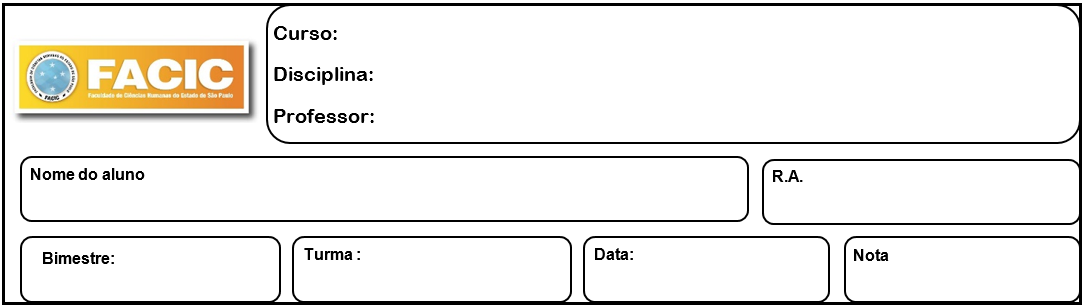
\includegraphics[width=1\linewidth]{cabecalho_FACIC}
%\end{figure}

%\vspace{-5.25cm}\hspace{5.5cm}{\textbf{ADMINISTRAÇÃO e CIÊNCIAS CONTÁBEIS}}

%\vspace{.21cm}\hspace{6.1cm}{\textbf{ÁLGEBRA LINEAR}}

%\vspace{.25cm}\hspace{6.1cm}{\textbf{FUMACHI}}

%\vspace{2.1cm}\hspace{1.1cm}{\textbf{2º Bimestre}}
%\hspace{6.3cm}{\textbf{}}

%\vspace{0.4cm}
\begin{center}\textbf{\Large{Disciplina de Álgebra Linear - 2 Adm e 2 CC \\ Prof. Fumachi \\ \vspace{0.5cm} Atividade 02}}\end{center}
\begin{center}\large{Data limite de entrega: 18/04/2020}\end{center}
%\textbf{Orientações:}
%\begin{enumerate}[label=\alph*,nosep]
%	\item[a)]{A avaliação é INDIVIDUAL;}
%	\item[b)]{NÃO é permitido a comunicação com outros colegas/amigos durante a avaliação;}
%	\item[c)]{NÃO é permitido durante a avalição utilizar qualquer equipamento elétrico, eletrônico, EXCETO calculadora PRÓPRIA;}
%	\item[d)]{NÃO é permitido emprestar materiais dos e/ou para os colegas, mesmo que tenha terminado a avaliação;}
%	\item[e)]{O não cumprimento de um, ou mais, dos itens (a-d), acarretará na anulação da avaliação e será atribuída a nota 0 (zero);}
%	\item[f)]{O entendimento da questão/enunciado faz parte da avaliação, ou seja, não haverá explicações do professor;}
%	\item[g)]{As respostas das questões devem ser feitas apenas no espaço destinado a mesma e devem ser feitas a tinta (preta ou azul). Respostas com rasuras, não legíveis ou feitas a grafite serão anuladas.}
%\end{enumerate}
	
\par\noindent\rule{\textwidth}{1pt}
%\textbf{{Questões}}

\vspace{0.25 cm}

\noindent 1. Calcule $\mathrm{det}(\mathbb{A})$ sendo $\mathbb{A} = \left[ \begin{matrix} 1&2&3 \\ 4&2&1 \\ -1&2&0 \end{matrix} \right]$

\noindent 2. Calcule $\mathbb{A} \cdot \mathbb{B}$ sendo $\mathbb{A} = \left[ \begin{matrix} 1&2&3 \\ 4&2&1 \\ -1&2&0 \end{matrix} \right]$ e $\mathbb{B} = \left[ \begin{matrix} 0&2&2 \\ 1&3&1 \\ -1&4&1 \end{matrix} \right]$.

\noindent 3. \um Calcule $\mathbb{A} \cdot \mathbb{B}$ sendo $\mathbb{A} = \left[ \begin{matrix} 1&2&3 \end{matrix} \right]$ e $\mathbb{B} = \left[ \begin{matrix} 0 \\ 1 \\ -1 \end{matrix} \right]$

\noindent 4. Calcule $\mathrm{det}(\mathbb{A})$ sendo $\mathbb{A} = \left[ \begin{matrix} 1&3&0&1 \\ 4&2&0&0 \\ -1&3&0&1 \\ 4&3&2&0 \end{matrix} \right]$.

\noindent 5. Calcule a área da figura abaixo:

\begin{tikzpicture}[scale=1.0]
% Estilos
\tikzstyle {every pin} = [ rectangle, rounded corners=1pt, font=\large ]
\begin{axis}
[
grid, grid style=dashed,
grid = both,
ymin=-.5,ymax=6.2,
xmin=-.5,xmax=6.2,
%xlabel=$x$,
%ylabel=$f(x)$,
width=10cm,
axis on top=true,
axis x line=middle,
axis y line=middle,
%transpose legend,
%legend columns = 1,
%legend style = {at={0.5,-.1},anchor=north}
legend pos= north east, %outer
]
%\draw[blue, very thick] (50,50) rectangle (550,550);
\path[draw, fill=gray!20, very thick] (50,50) rectangle (550,550);
%\draw[orange, ultra thick] (150,150) -- (450,150) -- (150,450) -- cycle;
\path[draw, fill=white!10, ultra thick] (150,150) -- (450,150) -- (150,450) -- cycle;
% Desenha a função
%\addplot [blue,line width = 1, smooth, domain=-1:3] {2*x +1}; %\addlegendentry{x}

% Pontos de interesse
\node [fill=none, circle, scale=0.75, pin=45:{$A_h$}] at (axis cs: 3.5,3.5) {};
%\node [fill=red, circle, scale=0.5, pin=180:{$(0,1)$}] at (axis cs: 0,1) {};
%\node [fill=blue, circle, scale=0.1, pin=135:{$f(x)=2x+1$}] at (axis cs: 2.75,6.5) {};
%\legend {$f(x)=2x+1$}
\end{axis}
\end{tikzpicture}
%\vspace{12.5cm}
%\resposta
%--------------------------------------

%\noindent 2. Classifique as sentenças abaixo em Verdadeiro (V) ou Falso (F):
%\vspace{.3cm}
%\begin{enumerate}[label=\alph*,nosep]
%	\item[2.1.]{(\qquad) O elemento neutro da soma de matrizes é a matriz nula.}
%	\item[2.2.]{(\qquad) O elemento neutro da multiplicação de matrizes é a matriz identidade.}
%	\item[2.3.]{(\qquad) A matriz identidade é uma matriz quadrada onde os elementos da diagonal principal são iguais a 1 e o restante iguais a 0.}
%	\item[2.4.]{(\qquad) Um sistema linear quando possui solução única ele é chamado de Sistema Possível e Determinado.}
%	\item[2.5.]{(\qquad) Um sistema linear pode ser classificado como SPI, SPD e SI.}
%	\item[2.6.]{(\qquad) O método de Cramer para resolver sistemas lineares possui falhas.}
%	\item[2.7.]{(\qquad) O método de Gauss para resolver sistemas lineares é conhecido, também, como método do escalonamento.}
%	\item[2.8.]{(\qquad) A matriz ampliada é usada no método de Gauss.}
%	\item[2.9.]{(\qquad) Na regra de Cramer, a matriz principal é uma matriz composta pelos coeficientes de um sistema linear.}
%	\item[2.10.]{(\qquad) O objetivo do método de Gauss para resolver sistemas lineares é obter uma matriz triangular inferior.}
%\end{enumerate}
%--------------------------------------

%\vspace{1cm}
\par\noindent\rule{\textwidth}{1pt}
Fim da Atividade 02.


\end{document}